\ifx\isEmbedded\undefined
\documentclass[12pt]{article}
	
% FONT RELATED
%\usepackage{times} %Move to times font
\usepackage[labelfont=bf,textfont=it]{caption}


% LINKS, PAGE OF CONTENT, REF AND CROSS-REF, HEADERS/FOOTERS
\usepackage{hyperref}
\hypersetup{
    colorlinks,
    citecolor=black,
    filecolor=black,
    linkcolor=black,
    urlcolor=black
}
%\usepackage[breaklinks=true]{hyperref}
\usepackage{fancyhdr}
\usepackage{acronym}

% FIGURES, GRAPHICS, TABLES
\usepackage{graphicx}
\usepackage{parskip}
\usepackage{subfigure}

% COLOURS, TEXT AND FORMATTING
\usepackage{array}
\usepackage{color}
\usepackage{setspace}
\usepackage{longtable}
\usepackage{multirow}

% ADVANCED MATHS, PSEUDO-CODE
\usepackage{amsmath}
\usepackage{alltt}
\usepackage{amsfonts}
\usepackage{listings}
\usepackage{amsmath}

% BIBLIOGRAPHY
\usepackage[authoryear]{natbib}
\bibpunct{(}{)}{;}{a}{}{,}

% USE IN DISSER:

\setlength\oddsidemargin{1.5cm}
\setlength\evensidemargin{5cm}

\setlength\textheight{9.0in}
\setlength\textwidth{5.1in}

% indent at each new paragrapg
\setlength\parindent{0.5cm}

\setlength\topmargin{-0.2in}
\renewcommand{\baselinestretch}{1.3}

%REPORT

%\setlength\oddsidemargin{1cm}
%\setlength\evensidemargin{0.3in}
%%\setlength\headsep{2.5in}
%
%\setlength\textheight{9.0in}
%\setlength\textwidth{5.5in}
%
%% indent at each new paragrapg
%\setlength\parindent{0.5cm}
%
%%\setlength{\parskip}{10.5ex}
%
%\setlength\topmargin{-0.2in}

%\newcommand{\HRule}{\rule{\linewidth}{0.5mm}}
\newcommand{\HRule}{\rule{\linewidth}{0.0mm}}

%% macros
\newcommand{\RR}{\mathbb{R}} 
\newcommand{\pt}[1]{\mathbf{#1}} 

% Color definitions (RGB model)
\definecolor{ms-comment}{rgb}{0.1, 0.4, 0.1}
\definecolor{ms-question}{rgb}{0.8, 0.2, 0.2}
\definecolor{ms-new}{rgb}{0.2, 0.4, 0.8}

\newcommand\red[1]{{\color{red}#1}}
\newcommand\blue[1]{{\color{blue}#1}}
\newcommand\comment[1]{{\iffalse #1 \fi}}

\setcounter{secnumdepth}{3}
\setcounter{tocdepth}{3} 

\graphicspath{{../img/}}
\begin{document}
\tableofcontents
\pagebreak

\section*{List of Acronyms}
\addcontentsline{toc}{section}{List of Acronyms}

\begin{acronym}[NURBS ]
\acro{AABB}{Axis Aligned Bounding Box}
\acro{ADF}{Adaptively sampled Distance Field}
\acro{BRep}{Boundary Representation}
\acro{BReps}{Boundary Representations}
\acro{BVH}{Bounding Volume Hierarchy}
\acro{CAD}{Computer-Aided Design}
\acro{CSG}{Constructive Solid Geometry}
\acro{FRep}{Function Representation}
\acro{GPU}{Graphics Processing Unit}
\acro{MVC}{Mean Value Coordinates}
\acro{NURBS}{Non-Uniform Rational B-Spline}
\acro{OBB}{Oriented Bounding Box}
\acro{PCA}{Principal Component Analysis}
\acro{RBF}{Radial Basis Function}
\acro{SAH}{Surface Area Heuristic}
\acro{SDF}{Signed Distance Field}
\acro{STTI}{Space Time Transfinite Interpolation}
\acro{SARDF}{Signed Approximate Real Distance Functions}
\acro{TI}{Transfinite Interpolation}
\end{acronym}

\pagebreak
\fi

\section{Cloth Model}\label{sec_model}
In order to simulate a piece of cloth, it has to be modelled some way in the computer. The implemented software is based on the particle-based model described in the first report. This entails discretizing the cloth into point masses or particles, as opposed to using FEM-based approaches (for an overview of existing techniques, see \citep{star_magn}). The forces on the particles are simulated by the software using springs, resulting in a classical mass-spring model. This is very similar to the models used in research e.g. \citep{provot_model, bridson_2002, choiko, position_based_dyn}, ...).\\

The configuration of the particles and springs in the author's implementation is as in \citep{robust_friction_2007}: every vertex of the triangle mesh is turned into a particle. The edges of every triangle are turned into structural springs, and bending springs are added in between the different vertices of adjacent triangles. The configuration of springs and particles is shown in image \ref{model_spring}. This allows for random objects to be easily read in as cloth. This is an improvement over the regular grid of methods such as the one in \cite{provot_model}, since converting random objects to such a regular grid is non-trivial, see image \ref{model_regular}. Hence, the resulting software allows to read in an OBJ file for the cloth to be simulated, as long as the mesh is triangular, as shown in image \ref{model_dress}. The code that reads in an obj file and turns it into the described model can be found in the {\bf ClothFactory} class (both .h and .cpp files). An important remark is that, in order to speed-up finding adjacent triangles, the {\bf TriangleRenderStructure} is used. This structure will be discussed later on.\\

\begin{figure}[!htb]
  \centering
  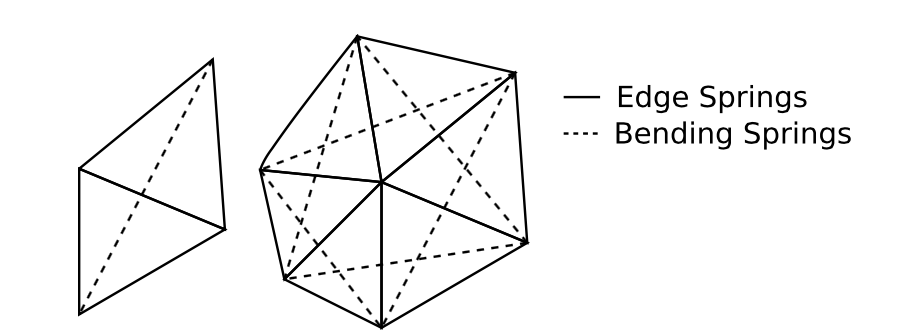
\includegraphics[width=4in,natwidth=366,natheight=166]{img/springConfig.png}
  \caption
   {Clarification of the way particles and springs are configured in the student's software. Every vertex the mesh is a particle, every edge is a structural spring, and adjacent triangles are connected with bending springs. Image by \cite{robust_friction_2007}.}
 \label{model_spring}
\end{figure}

\begin{figure}[!htb]
  \centering
  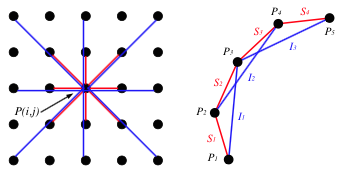
\includegraphics[width=4in,natwidth=366,natheight=166]{img/mass_spring_model.png}
  \caption
   {Regular grid for cloth as presented in \cite{provot_model}. Random objects do typically not have a regular layout of vertices. One could wonder how to connect bending springs if the grid is not regular.}
 \label{model_regular}
\end{figure}

\begin{figure}[!htb]
  \centering
  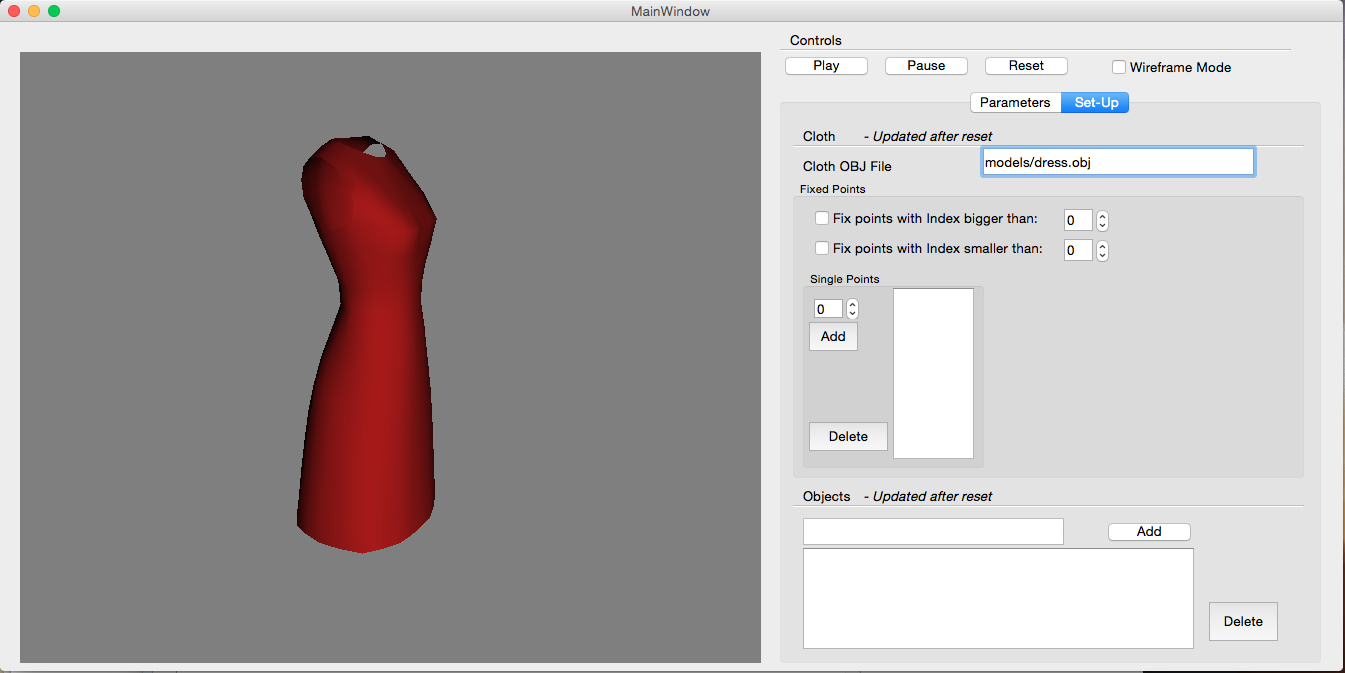
\includegraphics[width=4in,natwidth=366,natheight=166]{img/dress_model.png}
  \caption
   {The student's software showing an example of a triangular mesh read in. In this case a dress modelled by fellow student Stuart Macbean.}
 \label{model_dress}
\end{figure}

The springs exert forces following the classic spring formula, Hooke's law. Using the notation of \cite[chap. 7 ]{parent_book}, the springs exerts following forces:
\begin{equation}
\begin{split}
F_{\mathrm{spring}} = &- k_s (L_c - L_r) \frac{p_2 - p_1}{||p_2 - p_1||},\\
F_{\mathrm{damper}} = &- k_d (\dot{p_2} - \dot{p_1}) \cdot (\frac{p_2 - p_1}{||p_2 - p_1||}) (\frac{p_2 - p_1}{||p_2 - p_1||}).
\end{split}
\end{equation}
Where $p_2$ and $p_1$ are the positions of the particles connected to either end of the spring, $F_{\mathrm{spring}}$ and $F_{\mathrm{damper}}$ are the forces exerted by the spring and its damper respectively, $L_c$ is the current length of the spring (i.e. distance between $p_2$ and $p_1$) and $L_r$ is the rest length of the spring. The spring can be controlled with the two constants $k_s$, the spring constant, and $k_d$, the damper constant.\\

The implementation of these formulas can be found in the {\bf Spring} class. These forces also have to be derived into jacobian, since the student implemented implicit integration. The correct jacobian for the spring force according to the position of the particles $i$ and $j$ is as follows \citep{choiko}:
\begin{equation}
\frac{\delta F_{\mathrm{spring}}}{\delta x} = k_s \frac{p_{ij}p_{ij}^T}{p_{ij}^Tp_{ij}} + k_s (1 - \frac{L_r}{|p_{ij}|})(I - \frac{p_{ij}p_{ij}^T}{p_{ij}^Tp_{ij}}).
\end{equation}
Here all symbols stay the same as in the force equations. Furthermore, $p_{ij}$ now represents the difference between the position of particle $i$ and of position $j$, the particles on either end of the spring ($p_{ij} = p_j - p_i$). $I$ is the identity three by three matrix. The jacobian according to velocity is the identity matrix multiplied with the damping constant, as damping is the only force term depending on the velocity rather than the position. For this reason it does not appear in the positional jacobian. Implementation of both Jacobians can be found in the {\bf Spring class}.\\

Some external forces were also implemented by the student: a gravity-like force (constant acceleration), drag (a force counteracting the overall velocity of the particle) and wind. The implemented formulas for these forces are:
\begin{equation}
\begin{aligned}
F_{gravity} = m a_{grav}\\
F_{drag} = - d_c v^2\\
F_{wind} =  w_c (n \cdot W)
\end{aligned}
\end{equation}
For $F_{gravity}$ we multiply the gravitional acceleration $a_{grav}$ with the mass $m$ of the particle, $F_{drag}$ is computed from the velocity of the particle $v$ and the drag constant $d_c$ and $F_{wind}$ can be found using (the absolute value of) the dot product of the surface normal in the particle $n$ with the direction of the wind $W$, and multiplying it by a wind constant $w_c$. The implementations of these forces can be found in the {\bf GravityForce, DragForce and WindForce} classes respectively. Some random noise was added to the {\bf WindForce} to make it more realistic (see WindForce.cpp). Another force that was added was a constant force working on one particle, in the ConstantPull class.


\ifx\isEmbedded\undefined
% References
\addcontentsline{toc}{section}{References}
\bibliographystyle{../ref/harvardnat}
\bibliography{../ref/master}
\pagebreak
\end{document}
\fi